% textidote: ignore begin
\subsection{Database}\label{subsec:database}
% textidote: ignore end

The database option used is PostgresSQL~\cite{postgresql2024}, which is an open source relational database.
A relational database was chosen over a non-relational one due to the choice of back end batch processioning of the
imported CSV files.
In this way of processing, the implementation includes several tables in the database.

A figure of all the database tables can be seen in Figure~\ref{fig:database-diagram}.
The tables `order' and `order\_line' regards the final storage of user imported CSV files.
A non-relational database could also have been used for these, as the interdependencies of these tables are rather
simple.

\begin{figure}[H]
    \centering
    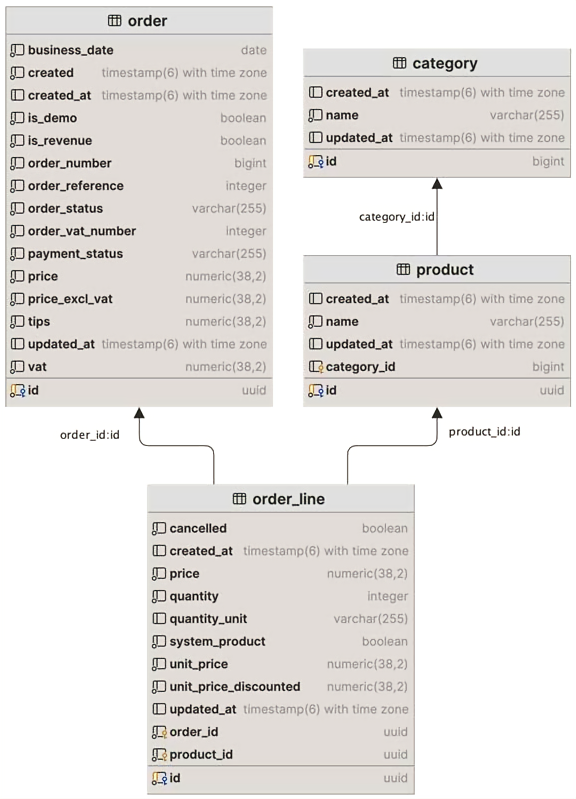
\includegraphics[width=.5\textwidth]{database-diagram}
    \caption{An overview of the physical database.
    }\label{fig:database-diagram}
\end{figure}

Furthermore, the database is run in its own container.
This is important as it makes potential maintenance easier, which is good practice in general.

% textidote: ignore begin
\subsubsection{Choice of relational database}\label{subsubsec:choice-of-relational-database}
% textidote: ignore end

During development, the PostgreSQL container could have been replaced with
% textidote: ignore begin
an H2
% textidote: ignore end
database~\cite{h22024} for two reasons:

\begin{itemize}
    \item The drawback with the
% textidote: ignore begin
    H2
% textidote: ignore end
    database is that it is an in-memory database.
    This means that the data will be lost on termination of the database instance.
    However, in development, the PostgreSQL Driver dependency was used, which starts and terminates the container
    containing the database on each reload of the back end.
    This results in the same drawback.
    \item The
% textidote: ignore begin
    H2
% textidote: ignore end
    database is all things considered easier and simpler to implement and work with.
    However, since the developers wanted to learn PostgreSQL and the handling thereof and because we would
    need it in the end anyway when deploying, we decided to go with the PostgreSQL database throughout the development.
\end{itemize}
